% !TeX root = Main.tex
Programový kód, kterým je realizována simulace šíření elektromagnetického pole, je proveden jako modul pro aplikaci Agros2D. Prostředí tohoto programu je patrné na obrázku \ref{obr:sim_agros2d}. Mezi základní prvky patří uprostřed umístěná pracovní plocha pro zadání geometrie řešeného problému a současně i prostor pro zobrazení výsledků. V~levé horní části se nachází informační okno o~daném řešeném problému včetně seznamu zadaných okrajových podmínek a materiálech. Pod tímto oknem je snadno dostupný postprocesor pro volbu zobrazení vyřešeného fyzikálního pole. Pravá oblast aplikace poskytuje možnost zobrazení hodnot konkrétních veličin v~požadovaném bodě.

\begin{figure}[!h]
	\centering
	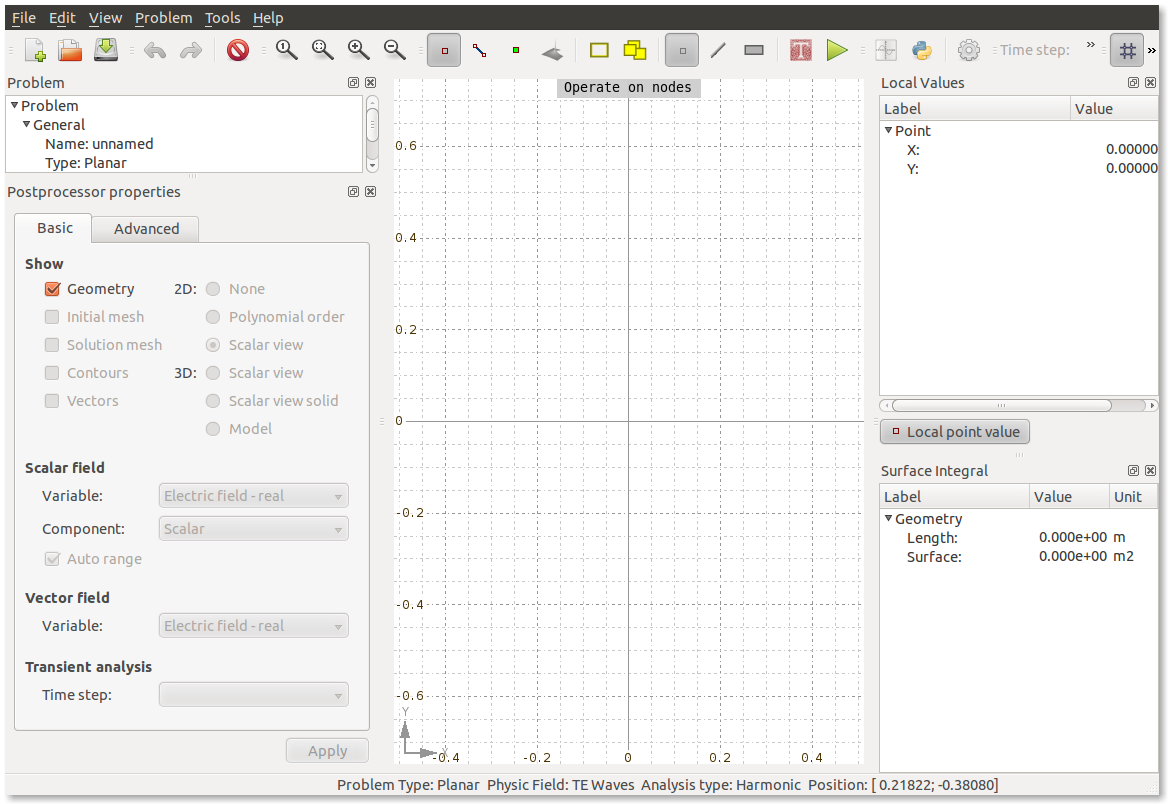
\includegraphics[width=14cm]{sim_agros2d.png}
	\caption{Základní pracovní rostředí programu Agros2D.}
	\label{obr:sim_agros2d}
\end{figure}

Samotný modul pro simulaci elektromagnetického pole tedy využívá z~programu Agros2D zmíněný preprocesor pro zadávání dat a postprocesor pro zobrazení výsledků ve 2D a 3D zobrazení. Vlastní numerické řešení zajišťuje knihovna Hermes2D a programový kód je obsažen v~ příslušném modulu. V~této kapitole jsou popsány výpočetní části, které se týkají především řešení vlnových rovnic, specifikace okrajových podmínek a zadávání materiálových konstant prostředí. 

\section{Metoda konečných prvků}
Základem samotné knihovny Hermes2D je numerické řešení pomocí tzv. metody konečných prvků neboli FEM (Finite Element Method). Historie spadá do první poloviny 20. století, kdy byly základy FEM popsány v~práci a Richarda Couranta (1943). Až v~roce 1953 byly rovnice popsány v~maticovém tvaru, což umožnilo řešení na počítačích a v~té době se FEM využívala v~leteckém průmyslu. K~jejímu šiřšímu využití v~dalších oborech však došlo až s~nástupem modernější výpočetní techniky v~průběhu 60. a 70. let. Například na problémy týkající se elektromagnetismu nebyla FEM použita dříve než v~roce 1968. V~současné době se však pomocí FEM výhodně řeší fyzikální problémy z~oborů statiky, dynamiky, akustiky, tepla, elektromagnetického pole, proudění, elektrostatiky a z~dalších vědeckých disciplín. 

Ačkoliv existují také jiné numerické metody řešení, například metoda konečných diferencí (FDM) nebo momentová metoda (MOM), které nejsou tak náročné na programovou implementaci, tak právě FEM je metodou nejvíce používanou. Důvodem je její všestrannost a výkonnost. Dalším aspektem je to, že programy vyvinuté pro konkrétní problémy mohou být snadno použity k~řešení příkladů v~naprosto jiném oboru pomocí drobných nebo dokonce žádných změn.

\subsection{Kroky řešení pomocí FEM}
Analýza jakéhokoliv problému prostřednictvím metody konečných prvků zahrnuje v~podstatě čtyři kroky:
\begin{itemize}
\item {Diskretizace oblasti na konečný počet prvků.}
\item {Vyjádření rovnic pro konkrétní prvek.}
\item {Sestavení prvků v~řešené oblasti.}
\item {Řešení získaných rovnic.}
\end{itemize}
Vlatní princip řešení a odvození příslušných rovnic je možné nalézt v~\cite[kap. 6.2]{num}, kde je FEM pro jednoduchost reprezentována na Laplaceově rovnici $\nabla^{2}V = 0$ .

\subsection*{Diskretizace}
Prvním krokem pro numerické řešení rovnic je rozdělení nekonečného objemu řešené oblasti na konečný počet prvků, tak jak je to naznačeno na obrázku \ref{obr:sim_diskretizace}.
\begin{figure}[!h]
	\centering
	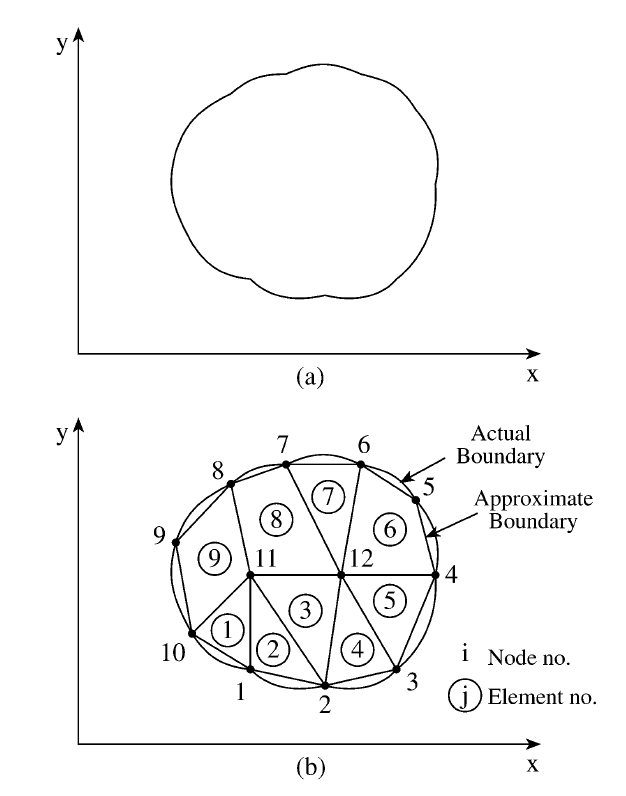
\includegraphics[width=13cm]{sim_diskretizace.png}
	\caption{Dělení řešené oblasti (a) na konečný počet diskretizačních prvků (b). \cite{num}}
	\label{obr:sim_diskretizace}
\end{figure}
Vlastní prvky, na které je oblast rozčleněna mohou mít libovolný tvar, ale typické tvary pro dvojdimenzionální problém jsou jsou naznačeny na obrázku \ref{obr:sim_prvky}.
\begin{figure}[!h]
	\centering
	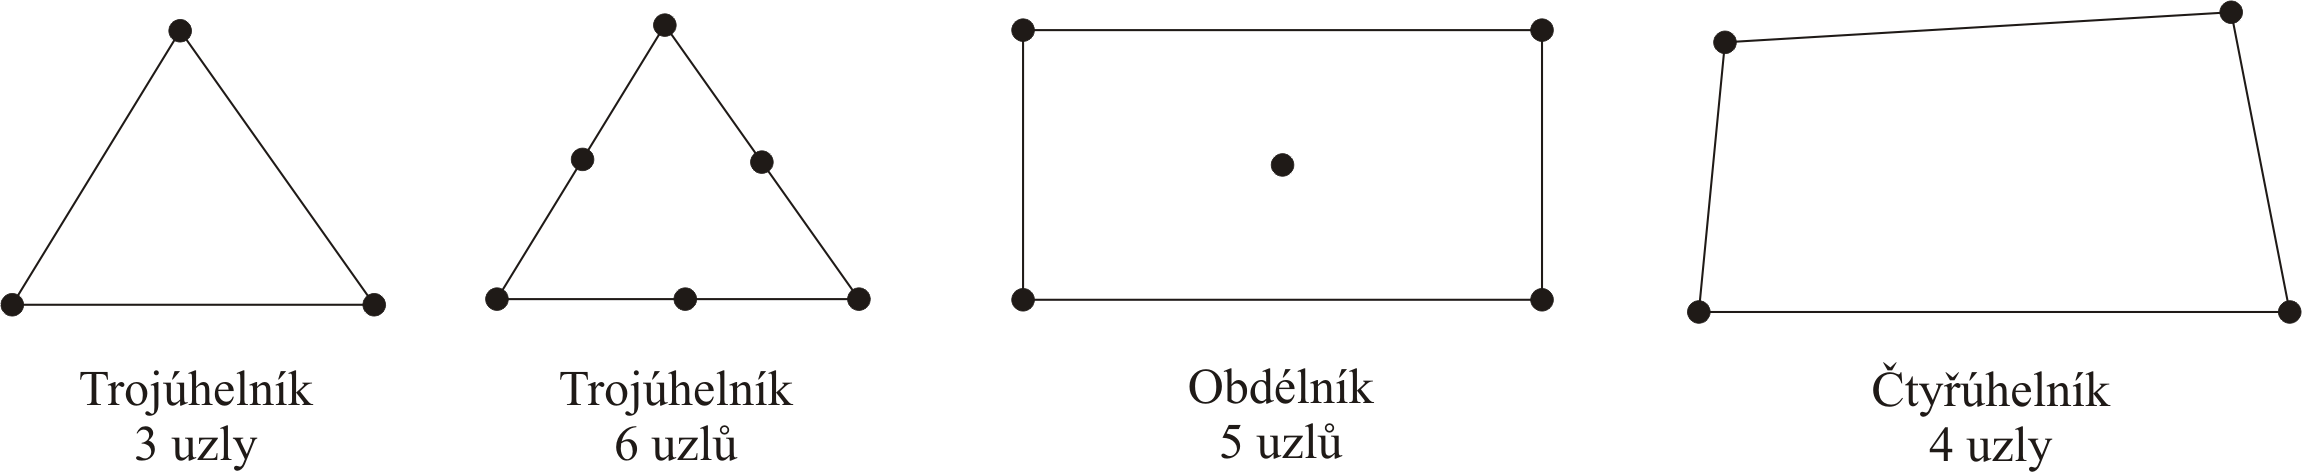
\includegraphics[width=9cm]{sim_prvky.png}
	\caption{Prvky diskterizace 2D oblasti. \cite{num}}
	\label{obr:sim_prvky}
\end{figure}

\subsection{Aproximované řešení}
Pro řešení diferenciální rovnice druhého řádu na obecné oblasti $\Omega$ je potřeba nejprve odvodit slabou formu. Ta představuje vynásobení rovnice testovací funkcí $v$ a poté integraci přes oblast řešení $\Omega$. Podrobný postup převodu pro Helmholtzovu rovnici (\ref{rce:sim_helmholtz_vychozi}) je blíže popsán v~podkapitole \ref{sec:sim_hermes2d}. Slabou formu výchozí řešené rovnice lze rozčlenit na bilineární a lineární členy. Bilineární člen $b(E_z,v)$ představuje levou stranu rovnic ve slabé formě a lineární člen $l(v)$ reprezentuje stranu pravou.
Aproximovaným řešením výchozí rovnice (\ref{rce:sim_kar_helmholtz_num}) je pak funkce $E_z$, pro kterou platí 
\begin{equation}
	b(E_z,v) = l(v),\qquad \mathrm{pro}\ E_z, v~\in V_{n}(\Omega),
	\label{rce:sim_aprox_reseni}
\end{equation}
kde $V_{n}(\Omega)$ představuje podprostor Hilbertova prostoru funkcí $H_{0}^{1}(\Omega)$. Řešení rovnice (\ref{rce:sim_aprox_reseni}) je možné zapsat jako lineární kombinaci bázových funkcí s~neznámými koeficienty, které je pro řešení potřeba nalézt
\begin{displaymath}
	E_z = \sum_{i=1}^{N}y_i v_i.
\end{displaymath}
Při položení bázových funkcí stejných jako testovací a dosazením do rovnice  (\ref{rce:sim_aprox_reseni}) obdržíme vztah
\begin{equation}
	\sum_{i=1}^{N}b(v_i,v_j)\cdot y_i = l(v_j),
	\label{rce:sim_aprox_reseni2}
\end{equation}
ze kterého vznikne systém algebraických rovnic s~neznámými koeficienty bázových funkcí, které aproximují řešení výchozí diferenciální rovnice na oblasti $\Omega$
\begin{equation}
	\vec S~\cdot \vec Y = \vec G.
	\label{rce:sim_aprox_matice}
\end{equation}
Matice $\vec S$ se označuje jako \uv{matice tuhosti}. Název má spojitost s~historií a pochází z~teorie elastických deformací. V~rovnici (\ref{rce:sim_aprox_matice}) je definována
\begin{displaymath}
	\vec S~= \{b(v_i,v_j) \}_{i,j = 1}^{N}.
\end{displaymath}
Vektor pravých stran lze zapsat
\begin{displaymath}
	\vec G = \{l(v_j) \}_{j = 1}^{N}
\end{displaymath}
a vektor neznámých koeficientů
\begin{displaymath}
	\vec Y = \{y_j \}_{j = 1}^{N}.
\end{displaymath}
Je zřejmé, že nalezení hledaných koeficientů $y_j$ spočívá v~řešení maticové rovnice ve tvaru
\begin{equation}
	\vec Y = \vec S~^{-1}\cdot \vec G.
	\label{rce:sim_aprox_inv_matice}
\end{equation}

\section{Řešení harmonické vlnové rovnice knihovnou Hermes2D} \label{sec:sim_hermes2d}
Vzhledem k~široké problematice elektromagnetických vln je potřeba pro jejich modelování zavést některé zjednodušení. 
\begin{itemize}
\item {\bf Harmonická analýza} - První předpokladem je řešení vlnové rovnice v~harmonickém tvaru (Helmholtzova rovnice)
\begin{equation}
	\nabla\times(\nabla\times\vecfaz E) +\faz k^{2}\vecfaz E = \mathrm{grad}\frac{\rho}{\varepsilon} + \mj\omega\mu\faz J_{\mathrm{ext}}.
    \label{rce:sim_helmholtz_vychozi} 
\end{equation}
\item {\bf Rovnoměrné rozložení náboje $\rho$} - Při této úvaze je v~řešené rovnici (\ref{rce:sim_helmholtz_vychozi}) člen $\mathrm{grad}\frac{\rho}{\varepsilon}$ roven nule.
\item {\bf Šíření vln v~kartézské souřadnicové soustavě v~jediném směru dle osy $z$} - Tento předpoklad platí pro planární problém.
\item {\bf Šíření vln v~polární souřadnicové soustavě má pouze tangenciální složku} - Uvažujeme pro osově symetrický problém.
\end{itemize}

\subsection{Kartézská souřadnicová soustava} \label{subsec:sim_kar}
Zavedením zjednodušujících předpokladů vycházíme z~rovnice ve tvaru
\begin{equation}
	\nabla^{2}\faz E_{(z)} +\faz k^{2}\faz E_{(z)} = \mj\omega\mu\faz J_{\mathrm{ext}},
	\label{rce:sim_kar_helmholtz_num} 
\end{equation}
platné na definované oblasti $\Omega$, na které známe okrajové podmínky a ve které chceme dostat výsledné řešení. Tím může být například vnitřní prostor vlnovodu nebo rezonátoru. Pro získání slabé formy k~rovnici (\ref{rce:sim_kar_helmholtz_num}) nejprve vyjádříme reálnou a imaginární složku
\begin{displaymath}
	\nabla^{2}(E_{z\Re} + \mj E_{z\Im}) + (\omega^{2}\varepsilon\mu - \mj\omega\mu\sigma)(E_{z\Re} + \mj E_{z\Im}) = \mj\omega\mu (J_{\mathrm{ext}\Re} + \mj J_{\mathrm{ext}\Im}),
\end{displaymath}
\begin{displaymath}
	\nabla^{2} E_{z\Re} + \mj\nabla^{2} E_{z\Im} + \omega^{2}\varepsilon\mu E_{z\Re} + \mj\omega^{2}\varepsilon\mu E_{z\Im} - \mj\omega\mu\sigma E_{z\Re} + \omega\mu\sigma E_{z\Im} = - \omega\mu J_{\mathrm{ext}\Im} + \mj\omega\mu J_{\mathrm{ext}\Re},
\end{displaymath}
kde reálnou část tvoří
\begin{equation}
	\Re : \nabla^{2} E_{z\Re} + \omega^{2}\varepsilon\mu E_{z\Re} + \omega\mu\sigma E_{z\Im} = - \omega\mu J_{\mathrm{ext}\Im}
	\label{rce:sim_kar_num_real} 
\end{equation}
a imaginární je vyjádřena
\begin{equation}
	\Im : \nabla^{2} E_{z\Im} + \omega^{2}\varepsilon\mu E_{z\Im} - \omega\mu\sigma E_{z\Re} = \omega\mu J_{\mathrm{ext}\Re}.
	\label{rce:sim_kar_num_imag} 
\end{equation}
Obě upravené rovnice (\ref{rce:sim_kar_num_real}) a (\ref{rce:sim_kar_num_imag}) je již možné převést do slabých forem, které splňují nulovou Dirichletovu a Neumannovu okrajovou podmínku. Postup převodu spočívá ve vynásobení parciálních diferenciálních rovnic testovací funkcí $v$ a v~následné integraci přes oblast řešení $\Omega$ 
\begin{equation}
	\Re : \int_{\Omega}\nabla^{2} E_{z\Re}\cdot v~\dif S~+ \omega^{2}\varepsilon\mu\int_{\Omega} E_{z\Re}\cdot v\dif S~+ \omega\mu\sigma\int_{\Omega} E_{z\Im}\cdot v\dif S~= - \omega\mu \int_{\Omega}J_{\mathrm{ext}\Im}\cdot v~\dif S,
	\label{rce:sim_kar_weak_odv_real} 
\end{equation}
\begin{equation}
	\Im : \int_{\Omega}\nabla^{2} E_{z\Im}\cdot v\dif S~+ \omega^{2}\varepsilon\mu\int_{\Omega} E_{z\Im}\cdot v\dif S~- \omega\mu\sigma\int_{\Omega} E_{z\Re}\cdot v\dif S~= \omega\mu \int_{\Omega}J_{\mathrm{ext}\Re}\cdot v~\dif S.
	\label{rce:sim_kar_weak_odv_imag} 
\end{equation}
V~dalším kroku se aplikuje 1. Greenova identita \cite[příloha A.2]{num} (integrace po částech pro vyšší řády) a tím se konečně získají slabé formy k~původním rovnicím (\ref{rce:sim_kar_num_real}) a (\ref{rce:sim_kar_num_imag})
\begin{displaymath}
\Re : \int_{\Gamma}\frac{\partial E_{z\Re}}{\partial n}\cdot v\dif l-\int_{\Omega}\nabla E_{z\Re}\cdot\nabla v~\dif S~+ \omega^{2}\varepsilon\mu\int_{\Omega} E_{z\Re}\cdot v\dif S~+ \omega\mu\sigma\int_{\Omega} E_{z\Im}\cdot v\dif
S~\end{displaymath}
\begin{equation}
	 = - \omega\mu \int_{\Omega}J_{\mathrm{ext}\Im}\cdot v~\dif S,
	\label{rce:sim_kar_weak_real} 
\end{equation}
\begin{displaymath}
\Im : \int_{\Gamma}\frac{\partial E_{z\Im}}{\partial n}\cdot v\dif l-\int_{\Omega}\nabla E_{z\Im}\cdot\nabla v\dif S~+ \omega^{2}\varepsilon\mu\int_{\Omega} E_{z\Im}\cdot v\dif S~- \omega\mu\sigma\int_{\Omega} E_{z\Re}\cdot v\dif S~\end{displaymath}
\begin{equation}
	= \omega\mu \int_{\Omega}J_{\mathrm{ext}\Re}\cdot v~\dif S.
	\label{rce:sim_kar_weak_imag} 
\end{equation}
První člen $\int_{\Gamma}\frac{\partial E_{z\Re}}{\partial n}\cdot v\dif l$ (respektive $\int_{\Gamma}\frac{\partial E_{z\Im}}{\partial n}\cdot v\dif l$) vyjadřuje Neumanovu okrajovou podmínku. Pokud je podmínka nulová, tak i tyto členy budou nulové. 

Levé strany rovnic představují bilineární členy daných slabých forem. Na pravých stranách se nacházejí členy lineární. K~první rovnici (\ref{rce:sim_kar_weak_real}) lze bilineární člen zapsat jako
\begin{equation}
	b(E_{z},v) = -\int_{\Omega}\nabla E_{z\Re}\cdot\nabla v~\dif S~+ \omega^{2}\varepsilon\mu\int_{\Omega} E_{z\Re}\cdot v\dif S~+ \omega\mu\sigma\int_{\Omega} E_{z\Im}\cdot v\dif
S~\label{rce:sim_kar_bilinear_real} 
\end{equation}
a lineární člen vztahem
\begin{equation}
	l(v) = - \omega\mu \int_{\Omega}J_{\mathrm{ext}\Im}\cdot v~\dif S.
	\label{rce:sim_kar_linear_real}
\end{equation}
U~rovnice druhé (\ref{rce:sim_kar_weak_imag}) jsou lineární a bilineární členy vyjádřeny
\begin{equation}
	b(E_{z},v) = -\int_{\Omega}\nabla E_{z\Im}\cdot\nabla v\dif S~+ \omega^{2}\varepsilon\mu\int_{\Omega} E_{z\Im}\cdot v\dif S~- \omega\mu\sigma\int_{\Omega} E_{z\Re}\cdot v\dif S,
	\label{rce:sim_kar_bilinear_imag}	
\end{equation}
\begin{equation}
	l(v) = \omega\mu \int_{\Omega}J_{\mathrm{ext}\Re}\cdot v~\dif S.
	\label{rce:sim_kar_linear_imag}
\end{equation}

\subsection{Polární souřadnicová soustava}
Řešení vlnové rovnice v~polárních souřadnicích vychází z~rovnice
\begin{equation}
	\nabla\times(\nabla\times\faz E_{\alpha}) +\faz k^{2}\faz E_{\alpha} = \mj\omega\mu\faz J_{\mathrm{ext}},
	\label{rce:sim_pol_helmholtz_num} 
\end{equation}
ve které je zavedeno zjednodušení, že výsledek má pouze tangenciální složku. Potom můžeme rovnici (\ref{rce:sim_pol_helmholtz_num}) snadno upravit. Nejprve vyjádříme vnitřní rotaci
\begin{displaymath}
	\nabla\times \frac{1}{r}\Bigg|
	\begin{array}{ccc}
\hat{r} & r\hat{\alpha} & \hat{z} \\
\frac{\partial}{\partial r} & \frac{\partial}{\partial \alpha} & \frac{\partial}{\partial z} \\
0 & r\faz E_{\alpha} & 0\\
\end{array}\Bigg| +\faz k^{2}\faz E_{\alpha} = \mj\omega\mu\faz J_{\mathrm{ext}},
\end{displaymath}
\begin{equation}
\nabla\times \Bigg[\hat{r}\bigg(-\frac{1}{r}\cdot\frac{\partial r\faz E_{\alpha}}{\partial z}\bigg) + \hat{\alpha}\bigg(0\bigg) + \hat{z}\bigg(\frac{1}{r}\cdot\frac{\partial r\faz E_{\alpha}}{\partial r}\bigg) \Bigg]+\faz k^{2}\faz E_{\alpha} = \mj\omega\mu\faz J_{\mathrm{ext}}.
	\label{rce:sim_pol_rotace1}
\end{equation}
Analogickým způsobem upravíme vnější rotaci ve vztahu (\ref{rce:sim_pol_rotace1})
\begin{displaymath}
	\frac{1}{r}\Bigg|
	\begin{array}{ccc}
\hat{r} & r\hat{\alpha} & \hat{z} \\
\frac{\partial}{\partial r} & \frac{\partial}{\partial \alpha} & \frac{\partial}{\partial z} \\
-\frac{1}{r}\cdot\frac{\partial r\faz E_{\alpha}}{\partial z} & 0 & \frac{1}{r}\cdot\frac{\partial r\faz E_{\alpha}}{\partial r}\\
\end{array}\Bigg| +\faz k^{2}\faz E_{\alpha} = \mj\omega\mu\faz J_{\mathrm{ext}},
\end{displaymath}
\begin{equation}
\Bigg[\hat{r}\bigg(\frac{1}{r}\cdot\frac{\partial}{\partial \alpha}\cdot\frac{1}{r}\frac{\partial r\faz E_{\alpha}}{\partial r}\bigg) + \hat{\alpha}\bigg(-\frac{\partial}{\partial z}\cdot\frac{1}{r}\cdot\frac{\partial r\faz E_{\alpha}}{\partial z} - \frac{\partial}{\partial r}\cdot\frac{1}{r}\cdot\frac{\partial r\faz E_{\alpha}}{\partial r}\bigg) + \hat{z}\bigg(\frac{1}{r}\cdot\frac{\partial}{\partial \alpha}\cdot\frac{1}{r}\frac{\partial r E_{\alpha}}{\partial z}\bigg) \Bigg]+\faz k^{2}\faz E_{\alpha} = \mj\omega\mu\faz J_{\mathrm{ext}}.
	\label{rce:sim_pol_rotace2}
\end{equation}
Ve výsledném vztahu (\ref{rce:sim_pol_rotace2}) zanedbáme všechny ostatní složky kromě té, která respektuje souřadnici $\hat{\alpha}$. Dostaneme rovnici
\begin{displaymath}
-\frac{\partial}{\partial z}\cdot\frac{1}{r}\cdot\frac{\partial r\faz E_{\alpha}}{\partial z} - \frac{\partial}{\partial r}\cdot\frac{1}{r}\cdot\frac{\partial r\faz E_{\alpha}}{\partial r}+\faz k^{2}\faz E_{\alpha} = \mj\omega\mu\faz J_{\mathrm{ext}},
\end{displaymath}
kterou upravíme do podoby
\begin{equation}
-\frac{\partial^{2}E_{\alpha}}{\partial z^{2}}-\frac{\partial^{2}E_{\alpha}}{\partial r^{2}}-\frac{1}{r}\cdot\frac{\partial E_{\alpha}}{\partial r} + \frac{E_{\alpha}}{r^{2}} +\faz k^{2}\faz E_{\alpha} = \mj\omega\mu\faz J_{\mathrm{ext}}.
	\label{rce:sim_pol_helmholtz_upravena}
\end{equation}
Tento vztah představuje vyjádření Helmholtzovy rovnice v~polárních souřadnicích, při uvažování výše uvedených předpokladů simulace. Pro zápis programového kódu k~vyřešení rozložení pole při osové symetrii je potřeba, stejným způsobem jako v~části \ref{subsec:sim_kar}, odvodit slabou formu k~rovnici (\ref{rce:sim_pol_helmholtz_upravena}) 
splňující Dirichletovu i Neumannovu okrajovou podmínku. 

\section{Okrajové podmínky}
Pro řešení diferenciálních rovnic popisující chování elektromagnetického pole v~dané oblasti $\Omega$ je třeba znát okrajové podmínky na hranicích. Účelem je specifikovat chování výsledné funkce, případně derivace této funkce, v~daných bodech ležících na okraji řešené oblasti. Při popisu fyzikálních polí pomocí diferenciálních rovnic se užívá Dirichletova, Neumannova nebo Newtonova (smíšená) okrajová podmínka.
\begin{itemize}
\item {\bf Dirichletova okrajová podmínka} - Předepisuje na hranici $\Gamma$ hodnotu funkce $E_{(z)}$, která může být obecně závislá na čase nebo na souřadnicích
\begin{displaymath}
	\faz E_{(z)}|_{\Gamma} = f_{Dir}(x,y,z,t). 
\end{displaymath}
\item {\bf Neumannova okrajová podmínka} - Na okraji řešené oblasti definuje tato podmínka hodnotu normálové derivace funkce $\frac{\partial E_{(z)}}{\partial n}$
\begin{displaymath}
	\frac{\partial \faz E_{(z)}}{\partial n}|_{\Gamma} = f_{Neu}(x,y,z,t). 
\end{displaymath}
\item {\bf Newtonova okrajová podmínka} - Neboli smíšená podmínka, kombinuje obě předchozí uvedené. Na hranici $\Gamma$ tak specifikuje kombinaci hodnoty funkce $E_{(z)}$ a její normálové derivace $\frac{\partial E_{(z)}}{\partial n}$
\begin{displaymath}
	\bigg(\frac{\partial \faz E_{(z)}}{\partial n} + \faz E_{(z)}\bigg)|_{\Gamma} = f_{New}(x,y,z,t). 
\end{displaymath}
\end{itemize}

\section{Možnosti zobrazení výsledků řešení}
Vlastnosti postprocessingu zobrazení v~programu Agors2D jsou velmi obsáhlé. Pomocí levého panelu v~pracovním okně (patrné na obrázku \ref{obr:sim_agros2d}) je možné vybrat zobrazení ve 2D nebo 3D prostoru a řadu dalších vlastností. 

Příslušné vztahy pro interpretaci výsledků je však potřeba implemetovat v~samostatném modulu, patřící k~jednotlivým polím. V~případě elektromagnetického pole nás bude zajímat především rozložení intenzit elektrického a magnetického pole, magnetické indukce, Poyntingova vektoru a ztrát. Programové kódy pro všechny zmíněné veličiny pole v~kartézských souřadnicích se nachází v~příloze \ref{kap:Program_kod}. 
 
\subsection*{Intenzita elektrického pole}
Hodnoty této veličiny v~řešených v~bodech na oblasti $\Omega$ odpovídají přímo řešení rovnice (\ref{rce:sim_kar_helmholtz_num}) v~kartézských souřadnicích nebo rovnice (\ref{rce:sim_pol_helmholtz_num}) v~polární souřadnicové soustavě.

\subsection*{Magnetická indukce}
Odvození vztahů pro zobrazení magnetické indukce vychází z~druhého Maxwellova zákona (\ref{rce:1MaxwR}), který má pro harmonické pole tvar
\begin{displaymath}
	\rot\vecfaz E = -\mj\omega\vecfaz B.
\end{displaymath}
Po úpravě rotace na levé straně výrazu pro jedinou složku $E_z$ dostaneme vztah
\begin{equation}
	\frac{\partial \faz E_z}{\partial y}\cdot\overrightarrow{\mathrm{i}} - \frac{\partial \faz E_z}{\partial y}\cdot\overrightarrow{\mathrm{j}} + 0\cdot\overrightarrow{\mathrm{k}} = -\mj\omega \faz B_x\cdot\overrightarrow{\mathrm{i}} - \mj\omega\faz  B_y\cdot\overrightarrow{\mathrm{j}} - \mj\omega\faz B_z\cdot\overrightarrow{\mathrm{k}},
	\label{rce:sim_zobrazeni_flux}
\end{equation}
ze kterého lze vyjádřit $x$-ová a $y$-ová složka magnetické indukce. $\faz B_z$ je podle rovnice (\ref{rce:sim_zobrazeni_flux}) nulová. Pro $\faz B_x$ tedy platí
\begin{displaymath}
	\faz B_x = -\frac{1}{\mj\omega}\frac{\partial E_z}{\partial y},
\end{displaymath}
kde po dosazení za $\faz E_z$ můžeme vyjádřit reálnou a imaginární složku magnetické indukce ve směru $x$, které lze pak implemetovat do modulu
\begin{equation}
	B_{x\Re} = -\frac{1}{\mj\omega}\frac{\partial E_{z\Im}}{\partial y}, \qquad \qquad B_{x\Im} = \frac{1}{\mj\omega}\frac{\partial E_{z\Re}}{\partial y}.
	\label{rce:sim_flux_x_re}
\end{equation}
Z~rovnice (\ref{rce:sim_zobrazeni_flux}) je pak dále možné stejným způsobem odvodit vztahy pro obě složky indukce ve směru $y$
\begin{equation}
	B_{y\Re} = \frac{1}{\mj\omega}\frac{\partial E_{z\Im}}{\partial x}, \qquad \qquad B_{y\Im} = -\frac{1}{\mj\omega}\frac{\partial E_{z\Re}}{\partial x}.
	\label{rce:sim_flux_y_im}
\end{equation}
Nakonec zbývá vyjádřit rozložení modulu magnetické indukce. Pro jeho velikost platí
\begin{displaymath}
	B = \sqrt{B_{x}^{2} + B_{y}^{2}} = \sqrt{B_{x\Re}^{2} + B_{x\Im}^{2} + B_{y\Re}^{2} + B_{y\Im}^{2}}.
\end{displaymath}

\subsection*{Intenzita magnetické pole}
Vztahy pro zobrazení magnetické složky pole s~výhodou vycházejí již z~vyjádřené magnetické indukce, neboť v harmonickém poli platí
\begin{displaymath}
\vecfaz H = \frac{1}{\mu} \vecfaz B.
\end{displaymath}
Je zřejmé, že veškeré výše odvozené vztahy (\ref{rce:sim_flux_x_re}) až (\ref{rce:sim_flux_y_im}) lze pouze podělit hodnotou permeability, která se nachází v~řešené oblasti. 

\subsection*{Poyntingův vektor}
Vektor vyjádřený vektorovým součinem intenzit elektrického a magnetického pole představuje plošnou hustotu výkonu na řešené oblasti $\Omega$
\begin{equation}
	\vecfaz N = \vecfaz E \times\vecfaz H\unit{[W/m^{2}]}.
	\label{rce:sim_poynting_vec}
\end{equation}
Úpravou rovnice (\ref{rce:sim_poynting_vec}) dostaneme vyjádření pro rozložení jednotlivé složky Poyntingova vektoru
\begin{equation}
	\faz N_x \cdot\overrightarrow{\mathrm{i}} + \faz N_y \cdot\overrightarrow{\mathrm{j}} + \faz N_z \cdot\overrightarrow{\mathrm{k}} = (-\faz E_z \faz H_y) \cdot\overrightarrow{\mathrm{i}} + \faz E_z \faz H_x \cdot\overrightarrow{\mathrm{j}} + 0 \cdot\overrightarrow{\mathrm{k}}.
	\label{rce:sim_poynting_vec_rozepsany}
\end{equation}
Je zřejmé, že $N_z$ je dle výrazu (\ref{rce:sim_poynting_vec_rozepsany}) nulový. Pro $x$-ovou složku platí
\begin{displaymath}
	\faz N_x = -\faz E_z \faz H_y,
\end{displaymath}
\begin{displaymath}
	\faz N_x = -(E_{z\Re} + \mj E_{z\Im})\cdot (H_{y\Re} + \mj H_{y\Im}),
\end{displaymath}
což ve výsledku vede na vztah
\begin{displaymath}
	\faz N_x = E_{z\Im} H_{y\Im} - E_{z\Re} H_{y\Re} - \mj (E_{z\Re} H_{y\Im} + E_{z\Im} H_{y\Re}).
\end{displaymath}
Pro Poyntingův vektor ve směru $y$ analogicky vychází
\begin{displaymath}
	\faz N_y = \faz E_z \faz H_x,
\end{displaymath}
\begin{displaymath}
	\faz N_y = E_{z\Re} H_{x\Re} - E_{z\Im} H_{x\Im} + \mj (E_{z\Re} H_{x\Im} + E_{z\Im} H_{x\Re}).
\end{displaymath}
Pro výslednou hodnotu Poyntingova vektoru na řešené oblasti $\Omega$ platí
\begin{displaymath}
	N = \sqrt{N_{x}^{2} + N_{y}^{2}} = \sqrt{(E_{z\Im} H_{y\Im} - E_{z\Re} H_{y\Re})^{2} + (E_{z\Im} H_{x\Im} - E_{z\Re} H_{x\Re})^{2}}.
\end{displaymath}

\subsection*{Jouleovy ztráty}
Rozložení ztrát v~řešené oblasti odpovídá součinu proudové husoty $J$ a hodnoty intenzity elektrického pole $E$ 
\begin{displaymath}
	P_j = \faz J \cdot \faz E = \sigma \faz E^{2} = \sigma \sqrt{E_{z\Re}^{2} + E_{z\Im}^{2}}\unit{[J/m^{3}]}.
\end{displaymath}

\section{Numerická integrace}
Výpočet určitých interálů, který se v~řešených vztazích vyskytují, je analyticky možný pouze v~určitých jednoduchých případech. Pro obecné funkce se integrace provádí numericky. Jednou z~možností je výpočet pomocí Gaussovy kvadratury.

Účelem je vypočítat numericky hodnodutu integrálu obecné funkce $g(\xi)$ na intervalu $x\in\langle a, b\rangle$,  pomocí aproximace výrazem
\begin{displaymath}
\sum_{i=0}^{n}\mathrm{w}_{t}[i]f(x_{i}),
\end{displaymath}
který se nazývá kvadraturní formule. Číslo $n$ představuje počet integračních bodů, hodnoty $\mathrm{w}_{t}[i]$ jsou příslušné váhové koeficienty uvedeného kvadraturního vzorce a $x_{i}$ se nazývají jeho uzly. 

Při výpočtu integrálu pomocí kvadraturní formule záleží tedy na volbě dělících bodů $x_{i}$ i koeficientů $\mathrm{w}_{t}[i]$. Právě princip Gaussovy kvadratury spočívá v~tom, jak vhodně zvolit $x_{i}$ a následně dopočítat $\mathrm{w}_{t}[i]$. Hodnoty uzlových bodů se pro jednorozměrný případ volí jako kořeny Legendrových polynomů
\begin{displaymath}
	P_{n}(x) = \frac{1}{2^{n}\cdot n!}\frac{\dif^{n}}{\dif x^{n}}[(x^{2} - 1)^{n}]
\end{displaymath}
a koeficienty $\mathrm{w}_{t}[i]$ jsou definovány
\begin{displaymath}
\mathrm{w}_{t}[i] = \frac{-2}{(n+2)P_{n+2}(x_i)P'_{n+1}(x_i)}.
\end{displaymath}
Více o~této metodě Gaussovy kvadratury je možné zjistit v~\cite{gk_tichy} nebo v~\cite{gk_kaw}.

\subsection{Numerický zápis rovnic kartézské souřadnicové soustavy}
\subsubsection*{Vyjádření členů rovnice (\ref{rce:sim_kar_weak_real})}
Bilineární člen rovnice, tj. vztah (\ref{rce:sim_kar_bilinear_real}) se ještě rozdělí části reprezentovaná reálnou a imaginární složkou. Nejprve vyjádříme zápis, který je v~programu označen indexem \uv{real\_real}. Rozepsáním operátoru $\nabla$ a numerickým řešením integrálů obdržíme výraz
\begin{equation}
	-\sum_{i=0}^{n}\mathrm{w}_{t}[i]\bigg(\frac{\partial E_{z\Re}}{\partial x}\cdot \frac{\partial v}{\partial x} + \frac{\partial E_{z\Re}}{\partial y}\cdot \frac{\partial v}{\partial y} \bigg) + \omega^{2}\varepsilon\mu\sum_{i=0}^{n}\mathrm{w}_{t}[i]\bigg(E_{z\Re}\cdot v\bigg),
	\label{rce:sim_kar_weak_real_real_num} 
\end{equation}
Obdobným způsobem postupujeme u~druhé složky bilineární části vyjádřené pomocí $E_{z\Im}$. Index funkce v~programu se změní na \uv{real\_imag}
\begin{equation}
 \omega\mu\sigma\sum_{i=0}^{n}\mathrm{w}_{t}[i]\bigg(E_{z\Im}\cdot v\bigg).
	\label{rce:sim_kar_weak_real_imag_num} 
\end{equation}
Nakonec je potřeba vyčíslit lineární část reálné složky, kterou reprezentuje rovnice (\ref{rce:sim_kar_linear_real})
\begin{equation}
 -\omega\mu\sum_{i=0}^{n}\mathrm{w}_{t}[i]\bigg(J_{\mathrm{ext}\Im}\cdot v\bigg).
	\label{rce:sim_kar_linear_real_num} 
\end{equation}


\subsubsection*{Členy rovnice (\ref{rce:sim_kar_weak_imag})}
Postup je naprosto totožný jako u~slabé formy reálné složky výchozí rovnice. Tudíž opět rozdělíme bilineární část na dvě části dle $E_{z\Re}$ a $E_{z\Im}$. Pro bilineární část (\ref{rce:sim_kar_bilinear_imag}) související s~indexem \uv{imag\_real} platí
\begin{equation}
 -\omega\mu\sigma\sum_{i=0}^{n}\mathrm{w}_{t}[i]\bigg(E_{z\Im}\cdot v\bigg)
	\label{rce:sim_kar_weak_imag_real_num} 
\end{equation}
a označení \uv{imag\_imag} odpovídá
\begin{equation}
	-\sum_{i=0}^{n}\mathrm{w}_{t}[i]\bigg(\frac{\partial E_{z\Im}}{\partial x}\cdot \frac{\partial v}{\partial x} + \frac{\partial E_{z\Im}}{\partial y}\cdot \frac{\partial v}{\partial y} \bigg) + \omega^{2}\varepsilon\mu\sum_{i=0}^{n}\mathrm{w}_{t}[i]\bigg(E_{z\Im}\cdot v\bigg).
	\label{rce:sim_kar_weak_imag_imag_num} 
\end{equation}
Imaginární lineární část (\ref{rce:sim_kar_linear_imag}) je reprezentovaná zápisem
\begin{equation}
 \omega\mu\sum_{i=0}^{n}\mathrm{w}_{t}[i]\bigg(J_{\mathrm{ext}\Re}\cdot v\bigg).
	\label{rce:sim_kar_linear_imag_num} 
\end{equation}

\subsection{Numerický zápis rovnic polární souřadnicové soustavy}
\subsubsection*{Reálná část vztahu (\ref{rce:sim_pol_helmholtz_upravena})}
Bilineární člen dané slabé formy s~indexem \uv{real\_real} lze po zavedení numerické integrace zapsat jako
\begin{displaymath}
-\sum_{i=0}^{n}\mathrm{w}_{t}[i]\bigg(\frac{\partial E_{\alpha\Re}}{\partial z}\cdot \frac{\partial v}{\partial z} + \frac{\partial E_{\alpha\Re}}{\partial r}\cdot \frac{\partial v}{\partial r} \bigg) - \frac{1}{r}\sum_{i=0}^{n}\mathrm{w}_{t}[i]\bigg(\frac{\partial E_{\alpha\Re}}{\partial r}\cdot v\bigg) +
\end{displaymath}
\begin{equation}
	 + \frac{1}{r^{2}}\sum_{i=0}^{n}\mathrm{w}_{t}[i]\bigg(E_{\alpha\Re}\cdot v\bigg) + \omega^{2}\varepsilon\mu\sum_{i=0}^{n}\mathrm{w}_{t}[i]\bigg(E_{\alpha\Re}\cdot v\bigg).
	\label{rce:sim_pol_bilinear_real_real} 
\end{equation}
Je zřejmé, že forma označená \uv{real\_imag} vyjde identicky jako v~případě kartézské souřadnicové soustavy, neboť člen $+\faz k^{2}\faz E_{\alpha}$ v~rovnici (\ref{rce:sim_pol_helmholtz_upravena}) je formálně stejný se vztahem (\ref{rce:sim_kar_helmholtz_num}). Platí tedy
\begin{equation}
 \omega\mu\sigma\sum_{i=0}^{n}\mathrm{w}_{t}[i]\bigg(E_{\alpha\Im}\cdot v\bigg).
	\label{rce:sim_pol_bilinear_real_imag} 
\end{equation}
Nakonec je potřeba zapsat lineární část reálné složky, která vyjde také identicky jako u~kartézské souřadnicové soustavy
\begin{equation}
 -\omega\mu\sum_{i=0}^{n}\mathrm{w}_{t}[i]\bigg(J_{\mathrm{ext}\Im}\cdot v\bigg).
	\label{rce:sim_pol_linear_real_num} 
\end{equation}

\subsubsection*{Imaginární část výrazu (\ref{rce:sim_pol_helmholtz_upravena})}
Slabým formám vycházející z~imaginární části z~původní rovnice (\ref{rce:sim_pol_helmholtz_upravena}) odpovídá vyjádření
\begin{equation}
 -\omega\mu\sigma\sum_{i=0}^{n}\mathrm{w}_{t}[i]\bigg(E_{\alpha\Re}\cdot v\bigg),
	\label{rce:sim_pol_bilinear_imag_real} 
\end{equation}
pro \uv{imag\_real}, což je opět ze stejného důvodu identické s~kartézskou souřadnicovou soustvou. Nakonec indexu \uv{imag\_imag} odpovídá
\begin{displaymath}
-\sum_{i=0}^{n}\mathrm{w}_{t}[i]\bigg(\frac{\partial E_{\alpha\Im}}{\partial z}\cdot \frac{\partial v}{\partial z} + \frac{\partial E_{\alpha\Im}}{\partial r}\cdot \frac{\partial v}{\partial r} \bigg) - \frac{1}{r}\sum_{i=0}^{n}\mathrm{w}_{t}[i]\bigg(\frac{\partial E_{\alpha\Im}}{\partial r}\cdot v\bigg) +
\end{displaymath}
\begin{equation}
	 + \frac{1}{r^{2}}\sum_{i=0}^{n}\mathrm{w}_{t}[i]\bigg(E_{\alpha\Im}\cdot v\bigg) + \omega^{2}\varepsilon\mu\sum_{i=0}^{n}\mathrm{w}_{t}[i]\bigg(E_{\alpha\Im}\cdot v\bigg).
	\label{rce:sim_pol_bilinear_imag_imag} 
\end{equation}
Imaginární lineární část je reprezentovaná opět identickým zápisem
\begin{equation}
 \omega\mu\sum_{i=0}^{n}\mathrm{w}_{t}[i]\bigg(J_{\mathrm{ext}\Re}\cdot v\bigg).
	\label{rce:sim_pol_linear_imag_num} 
\end{equation}